
\chapter{History}
This chapter summarizes the history of connectionist models used for graph processing. All these models originate from the feed-forward neural networks (FNNs). The history of neural networks begins in 1943 with the McCulloch–Pitts (MCP) neuron model, following with the Rosenblatt perceptron classifier in 1957. The feed-forward neural network model was developed during the following three decades and a conclusive state was reached in all major fields of related research until approximately 1988. The FNN model reached maturity in its field of application: classification and regression performed on unstructured positional samples of fixed size. In the '80s a new branch of the neural networks family began to develop - the recurrent neural networks (RNN). The RNN model is capable of processing sequences of varying length (potentially infinite), which makes them suitable for dealing with time-varying sequences or biological samples of various length~\cite{saha2006prediction}. However, a slightly different model had to be invented to properly process graph data.

\section{Hopfield networks}
One of the earliest attempts to classify structured data with neural networks was using the Hopfield networks~\cite{goulon2005hopfield}. A common application of a Hopfield network is an auto-associative memory, which learns to reproduce patterns provided as its inputs. (The task to be learned is the mapping $\bm{x}_i \Rightarrow \bm{x}_i$, where $\bm{x}_i$ is a pattern of fixed size $n$.) Afterwards, when a new sample is presented to the trained network, the network associates it with the most similar pattern it had learned. Subsequently, it was discovered, that by using a Hopfield network to reproduce a predefined successor of a pattern instead of the pattern itself, the network can be used as an hetero-associative memory, capable of reproducing sequences of patterns ($\bm{x}_i \Rightarrow \bm{x_{i+1}}$). The next step towards graph processing was to use Hopfield networks to learn the task of reproducing \emph{all} the successors (or predecessors) of a node, that is to learn the mapping $\bm{x}_i \Rightarrow succ[\bm{x}_i]$, where $x_i$ is the $i$th node label and $succ[\bm{x}_i]$ denotes a vector obtained by stacking together the labels of all the successors of node $\bm{x}_i$, one after another. For such task the maximum outdegree of a node (the maximum number of its successors) has to be known prior to the network training. $NIL$ patterns are used as extra successors labels whenever a considered node $\bm{x}_i$ has an outdegree smaller than the maximum value chosen. The last and somehow different application of Hopfield networks was to use a Hopfield network once again as an auto-associative memory, used for retrieving whole graphs. In such case the graph adjacency matrices ($N \times N$) are encoded into a network having $N(N - 1)/2$ neurons~\cite{goulon2005hopfield}, where $N$ is the number of nodes in a graph. To obtain an adequate generalisation, graphs isomorphic to the training set are generated and fed to the network~\cite{kree1988recognition}.

\section{RAAM}
The Recursive Auto-Associative Memory (RAAM) was introduced by Pollack in 1990~\cite{pollack1990recursive}. The RAAM model is a generalisation of the Hopfield network model~\cite{goulon2005hopfield}, providing means to meaningfully encode directed positional acyclic graphs (DPAGs). A distinctive feature of the RAAM model is that is can be used to encode graphs with labeled terminal nodes only. (The terminal nodes are nodes with outdegree equal to zero, that is nodes having no children. In the case of trees, leaves are terminal nodes.) That is, no node other than the terminal nodes of a graph may be labelled. No edge labels are permitted. The most straightforward domain of application for the RAAM model is thus natural language processing, where sentences can be decomposed to syntax graphs.\\
\noindent The RAAM model is capable of:
\begin{itemize}
	\item building compressed representation of structured data
	\item building meaningful representation: similar samples are represented in a similar way
	\item constrained generalisation: representing data absent in the training set
\end{itemize}
The RAAM model is composed of two units: \emph{compressor} and \emph{reconstructor}. Together they form a three-layer feed-forward neural network which works as an auto-associative memory. The \emph{compressor} is a fully connected two-layer neural network with $n$ input lines and $m$ output neurons. The number of output neurons, $m$ determines the size of a single encoded node representation. The number of input lines, $n$ must be a multiple of $m$, such that $n = k \cdot m$, where $k$ is the maximum outdegree of a node in the considered graphs. For each terminal node its representation consists of its original label. For each non-terminal node $i$ its representation, $\bm{x}_i$ is built by feeding the compressor with encoded representation of the $i$th nodes children.

To assure that the compressed representation is accurate and lossless, it is fed to the \emph{reconstructor}. The reconstructor is also a fully connected two-layer neural network, however it has $m$ input lines and $n$ output neurons. It is fed with compressed representations of nodes and is expected to produce the original data that was fed to the compressor. This procedure is repeated for all non-terminal nodes of a graph, until all encoded representations can be accurately decoded into original data. More precisely, the representation $\bm{x}_i$ of the $i$th node of the graph is given by Eq.~\ref{eq:raam_representation}, where $f$ denotes the function implemented by the compressor unit, $\bm{l}_i$ - the label of $i$th node, $\bm{x}_{ch[i]}$ - a vector obtained by stacking representations of all children of $i$th node one after another, $k$ - the maximum outdegree of a node in the graph.

\begin{equation}
\bm{x}_i = \left\{
\begin{array}{l l}
	\bm{l}_i & \quad \text{if $i$ is terminal} \\
	f(\bm{x}_{ch[i]}) & \quad \text{otherwise}
\end{array}
\right.
\label{eq:raam_representation}
\end{equation}

\noindent A sample graph that can be encoded using the RAAM model is presented in Fig.~\ref{fig:tree_for_raam}. The non-terminal nodes are enumerated for convenience only (only terminal nodes are labelled).

\begin{figure}
\begin{center}
	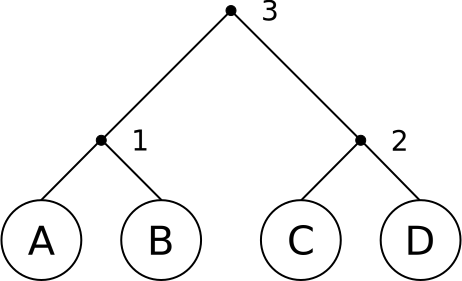
\includegraphics[scale=0.4]{img/tree_for_raam}
	\caption{A sample graph that can be processed using RAAM}
	\label{fig:tree_for_raam}
\end{center}
\end{figure}

\begin{figure}
\begin{center}
	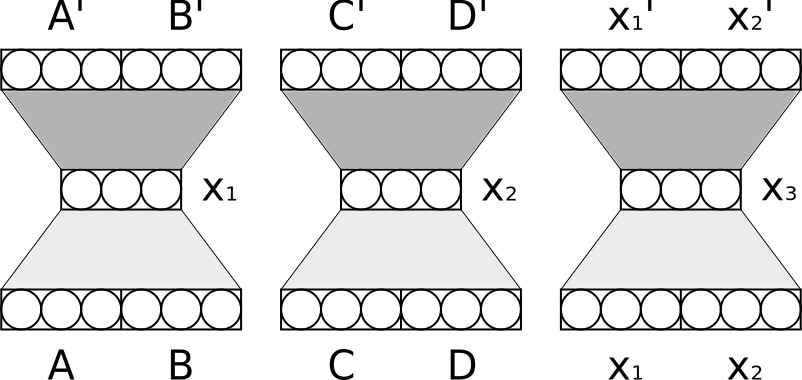
\includegraphics[scale=0.4]{img/raam1-3}
	\caption{Training set for the example graph}
	\label{fig:raam1-3}
\end{center}
\end{figure}

To encode the sample graph, the representations of nodes $1$ and $2$ must be built first. The representation of node $1$ is built by feeding the pair of labels $(A, B)$ to the compressor which encodes them into the representation $\bm{x}_1$. The representation $\bm{x}_1$ is then fed to the reconstructor, which produces a pair of labels $(A', B')$. If the resulting labels $A'$ and $B'$ are not similar enough to the original labels $A$ and $B$, the error is backpropagated through the compressor-reconstructor three-layer network. Similarly, the pair $(C, D)$ is processed by the same compressor-reconstructor pair and compressed into the representation $\bm{x}_2$. Then, the pair $(\bm{x}_1, \bm{x}_2)$ is once again fed to the compressor, which produces $\bm{x}_3$, the representation of the root node. This is also the compressed representation of the whole graph, from which the whole graph can be reconstructed by using the reconstructor unit. The training set, consisting of three label pairs, is presented in~Fig.~\ref{fig:raam1-3}. The light grey areas denote the compressor network, while the dark grey areas denote the reconstructor. Such a training set (or a larger one if the dataset consists of more than one graph) must be repeatedly processed by the RAAM model in the training phase. When the model is trained, the compression of the whole graph occurs as presented in~Fig.~\ref{fig:raam_compression}. Reconstruction of the graph is presented in~Fig.~\ref{fig:raam_reconstruction}. It is worth mentioning that a trained RAAM model can be used to process graphs with different structures.

\begin{figure}
\begin{center}
	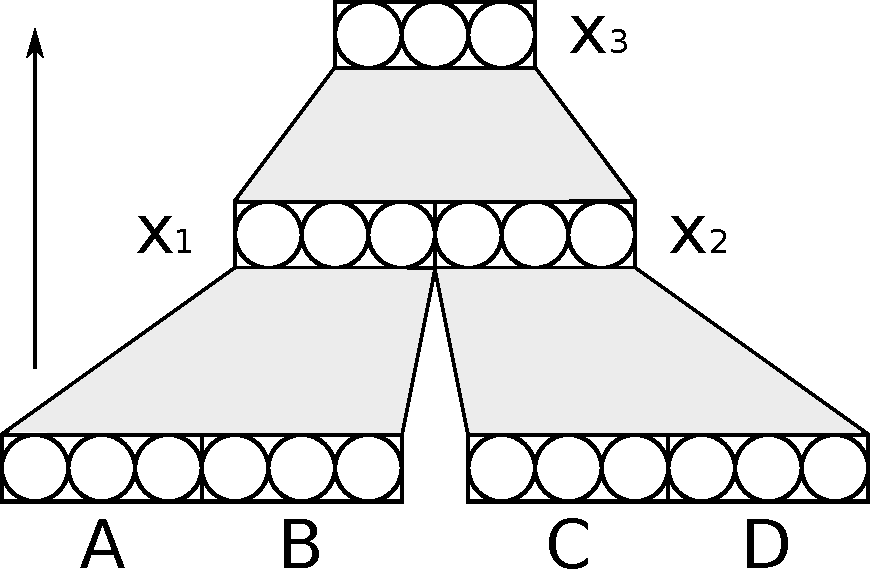
\includegraphics[scale=0.4]{img/raam_encode}
	\caption{Graph compression using trained RAAM model}
	\label{fig:raam_compression}
\end{center}
\end{figure}

\begin{figure}
\begin{center}
	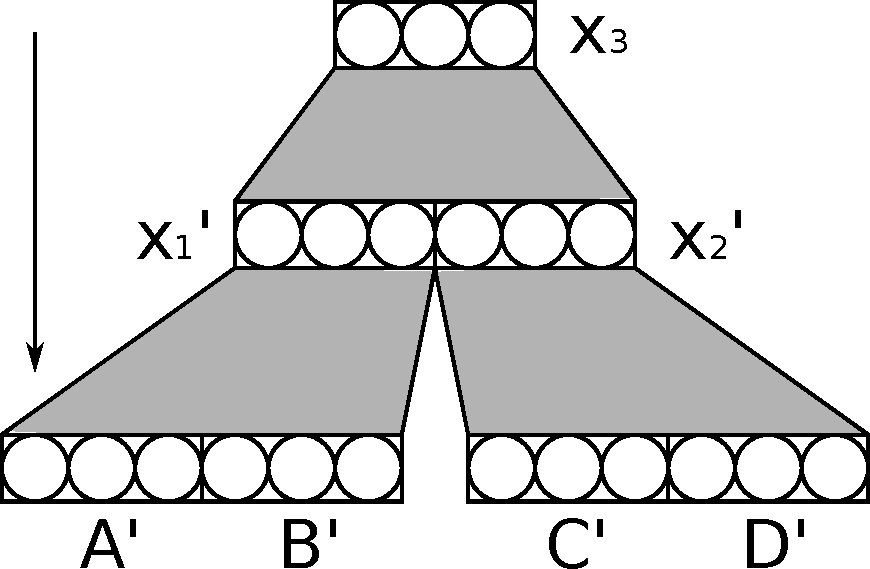
\includegraphics[scale=0.4]{img/raam_decode}
	\caption{Graph reconstruction from $\bm{x}_3$ using trained RAAM model}
	\label{fig:raam_reconstruction}
\end{center}
\end{figure}

A significant feature of the RAAM model is that a small reconstruction error in the case of non-terminal nodes may render the reconstruction of terminal nodes impossible. Therefore in the process of training a RAAM classifier it is necessary to set the acceptable reconstruction error value much smaller for the non-terminal nodes than for the terminal ones.

A major drawback of the RAAM model is the \emph{moving target} problem. That is, a part of the learning set (the representations $\bm{x}_1$ and $\bm{x}_2$ from the example) changes during training. In such a case the training phase may not converge to an acceptable state~\cite{goulon2005hopfield}. However, a different training schema is possible, based on the BPTS algorithm~\cite{goulon2005hopfield}. (An extensive description of the BPTS algorithm, \emph{encoding networks}, and the \emph{shared weights} technique is provided in the following chapters.) An encoding network is built out of identical instances of the compressor and reconstructor units (Fig.~\ref{fig:raam_tree}), with structure reflecting the structure of the processed graph (if the dataset consists of multiple graphs, such procedure is repeated for every graph in the dataset). All instances of the compressor unit share their weights and all instances of the reconstructor unit share their weights - which is called the \emph{shared weights} technique. The labels of terminal nodes are fed to the processing network and the resulting error can be backpropagated from the last layer using the Backpropagation Through Structure~\cite{kuchler1996inductive} algorithm (BPTS). It is worth mentioning, that the authors of such modified RAAM model propose using an additional layer of hidden neurons in the compressor and reconstructor units. In such case the light grey and dark grey areas on the figures would denote not only neuron connections between two layers, but also an additional hidden layer. Such modification allows to partially separate the problem of the data model complexity (i.e. how complex should the RAAM model be to properly compress the data) from the size of terminal node labels which affects directly the number of input lines to the compressor unit and thus the compressed representation size.

\begin{figure}
\begin{center}
	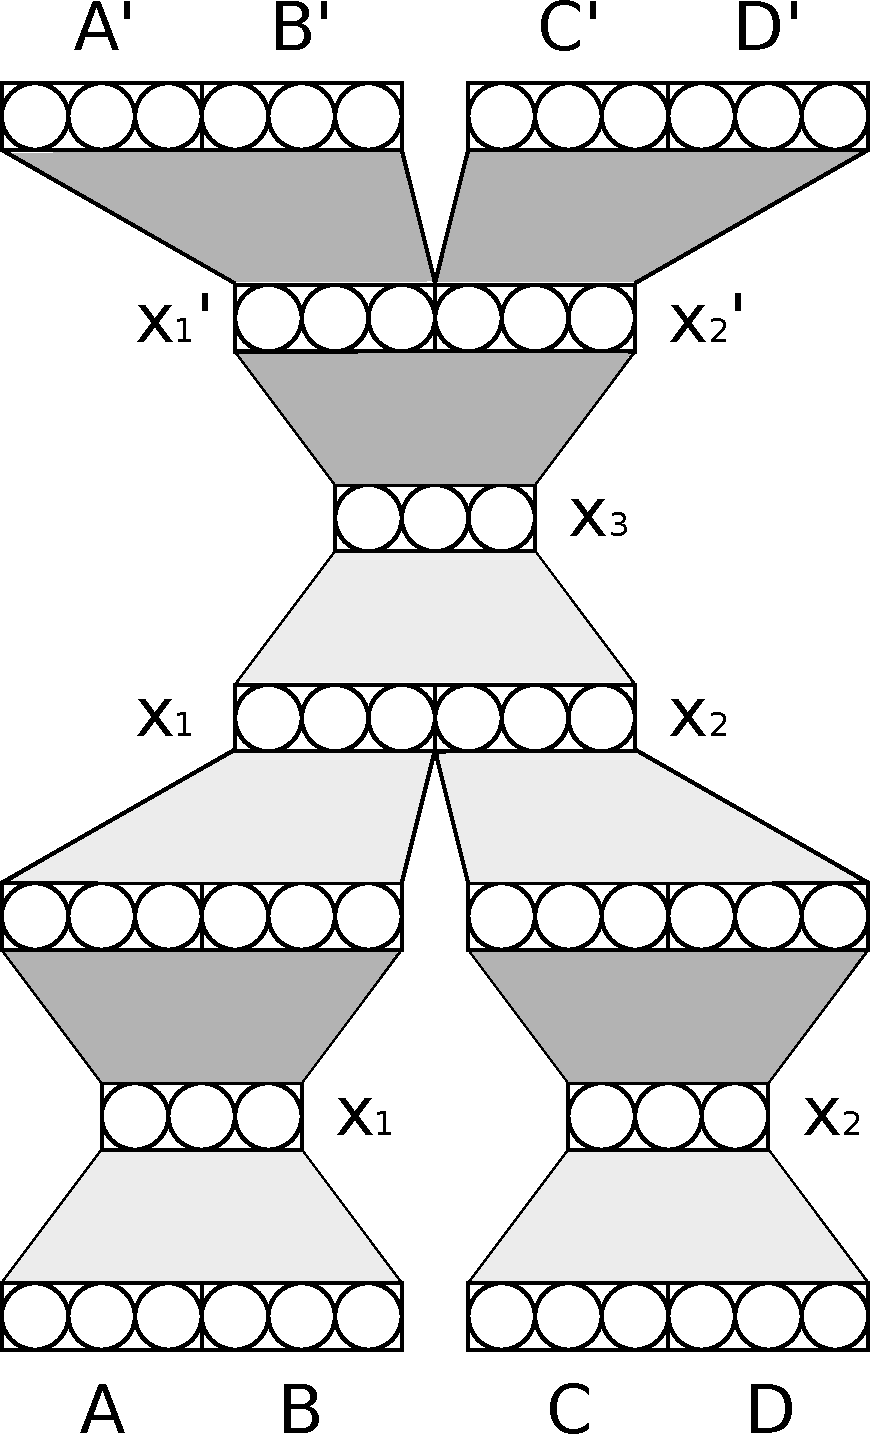
\includegraphics[scale=0.4]{img/raam_tree}
	\caption{Training RAAM using the BPTS procedure}
	\label{fig:raam_tree}
\end{center}
\end{figure}

The most important parameter of the RAAM model is the size of the compressed representation. On one hand, the size should be large enough to contain all the necessary compressed information about the encoded graph. On the other hand, it should be small enough for the compression mechanism to build a minimal representation, which stores only the necessary information about the dataset. If the size is too large, the trained model would store redundant information, memorizing the training set. This would result in a poor ability to process unseen data. Experiments with natural language syntax processing~\cite{pollack1990recursive} proved that when the size of the compressed representation is accurate for the problem, the RAAM model is showing some constrained generalisation properties. That is, unseen data with structure similar to the training set was processed properly by the trained RAAM model.

A drawback of the standard RAAM model is the termination problem. The reconstructor can't distinguish between terminal representations (node labels) and compressed representations, which should be further reconstructed. To solve this problem, an additional encoding neuron can be introduced (increasing the representation size by one), which takes a different value for terminal and non-terminal representations~\cite{stolcke1992tree}.

\section{LRAAM}
The most important constraint of the RAAM model is the fact that only terminal nodes of the processed graphs (DPAGs) can contain labels. This problem was addressed by the Labeling RAAM model~\cite{sperduti1994labelling} (LRAAM, 1994), which separated the concepts of node labels and node representations. In the RAAM model the terminal nodes are represented by their labels. The LRAAM model introduced the concept of \emph{pointers}, which was used to describe a node representation which has to be learnt, regardless of whether the node is terminal or not. The pointers are built by compressor units (FNN with two or more layers) and they are decoded into graph structure by reconstructor units. More precisely, the pointer to $i$th node of the graph is calculated according to Eq.~\ref{eq:lraam_pointer}, where $\bm{x}_i$ stands for pointer to the $i$th node, $f$ is the function implemented by the compressor unit, $\bm{l}_i$ is the $i$th node label, $\bm{x}_{ch[i]}$ is a vector obtained by stacking pointers to all children of $i$th node one after another and $k$ is the maximum outdegree of a node in the considered graph.

\begin{equation}
\bm{x}_i = f(\bm{l}_i, \; \bm{x}_{ch[i]})
\label{eq:lraam_pointer}
\end{equation}

Whenever a node outdegree is smaller than $k$ (especially in the case of terminal nodes), the missing child pointers are substituted by the $NIL$ pointer, a special value representing the lack of node. The value of the node label is stacked together with all the child pointers values to form an input vector which is fed to the compressor unit. The number of output neurons of the compressor unit (the size of a pointer $\bm{x}_i$) is $m$. Let's denote the size of the label $\bm{l}_i$ by $p$. The compressor unit must have $n = p + k \cdot m$ input lines which is also the number of reconstructor unit output neurons. The possibility of describing each graph node with its label provides a simple solution to the termination problem~\cite{sperduti1994labelling}. An additional value can be appended to each label, stating if the node is a terminal node or not. By using this method no change in the LRAAM model is needed.

Just like the RAAM model, the LRAAM model experience the problem of the \emph{moving target}. The same technique of \emph{shared weights} can be applied~\cite{goulon2005hopfield}, which results in building a large encoding network composed of identical units. A sample graph and the encoding network obtained by cloning the compressor and reconstructor units to reflect the sample graph structure are presented in Fig.~\ref{fig:lraam_tree}. As $A$ and $B$ are terminal nodes, their labels are fed to the compressor unit altogether with $NIL$ pointers representing the missing nodes. Then the compressed representation $\bm{x}_{A}$ is built for node $A$ and the compressed representation $\bm{x}_{B}$ is built for node $B$. The representations $\bm{x}_A$ and $\bm{x}_B$ are then fed altogether with the label $C$ to the compressor, to build the representation $\bm{x}_C$ of node $C$, which is also the compressed representation of the whole graph.

\begin{figure}
\begin{center}
	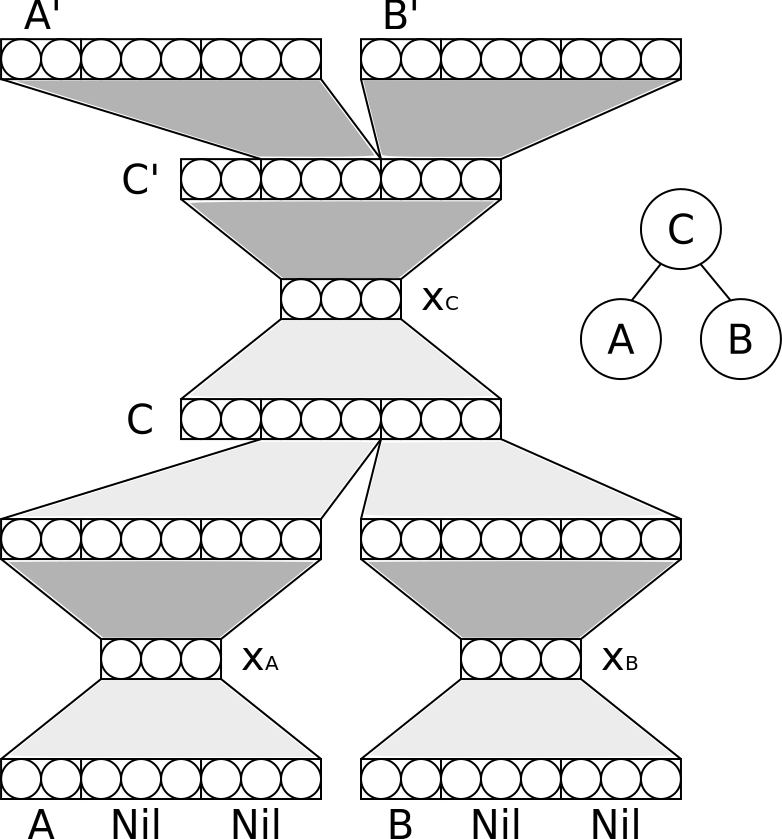
\includegraphics[scale=0.4]{img/lraam_tree}
	\caption{LRAAM encoding tree for the graph shown}
	\label{fig:lraam_tree}
\end{center}
\end{figure}

An extension of the LRAAM model exists for cyclic graphs~\cite{goulon2005hopfield}. Whenever an edge forming a cycle is found, it is converted to a single time unit delay (denoted by $q^{-1}$~\cite{frasconi1998general}). A sample cyclic graph and the resulting LRAAM model with one time delay was presented in Fig.~\ref{fig:lraam_tree_cycle}. The graph presented is similar to the graph used in the previous example, with the exception of the directed edge $A \Rightarrow C$. The additional edge forms a cycle so it must be represented as a time delay. Such an approach makes it possible to deal with cyclic graphs, however it is achieved at the expense of model simplicity. The shared weights technique made it possible to treat the encoding tree structure as a single feed-forward neural network with shared weights. However, after adding time delays the training of the network will have to consist of multiple time steps, repeated until convergence of the pointer values is reached.

\begin{figure}
\begin{center}
	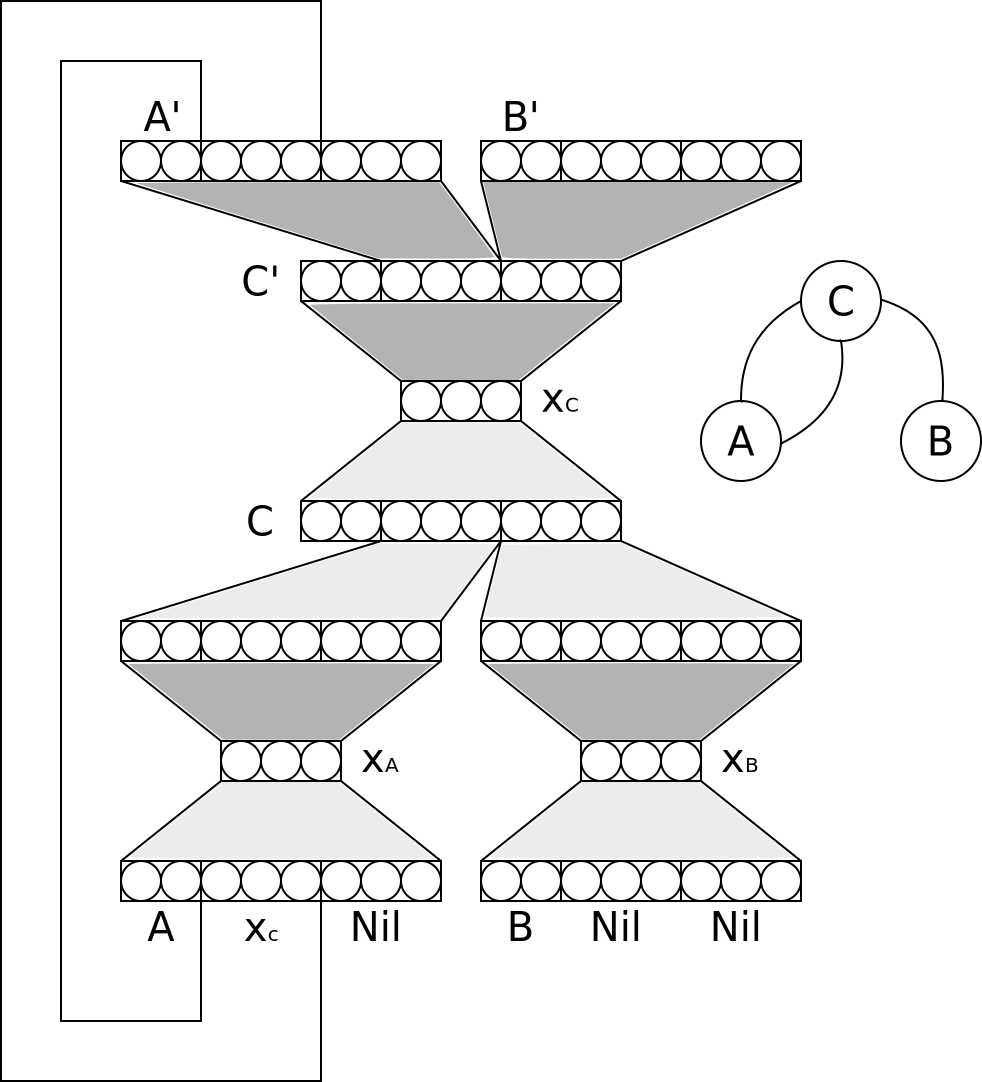
\includegraphics[scale=0.4]{img/lraam_tree_cycle}
	\caption{LRAAM encoding tree for the cyclic graph shown}
	\label{fig:lraam_tree_cycle}
\end{center}
\end{figure}

A distinctive feature of the LRAAM model is that a compressed representation is built for a given dataset (consisting of DPAGs) and the correctness of the representation is verified by mirroring the compression process and reconstructing the original data. When the obtained representation is accurate enough, the output of the LRAAM model is "frozen" and fed to a separate classifier which processes it and yields classification or regression results. The same applies to any new, unseen data, which is fed to the trained LRAAM model and, if the model was built correctly, is compressed into a meaningful representation. Such separation of representation building and processing can be attractive for two reasons. First, the LRAAM model parameters, such as the size of the representation, can be tuned in a straightforward manner by observing what is the minimal value below which the original data cannot be accurately reconstructed from the compressed vectors. Secondly, any vectorial classifier used for unstructured data can be used to process such compressed representation. On the other hand, it is often safe to presume that not all the data contained in node labels is crucial for the classification/regression process for which the compressed representation is needed. Such an approach lies beyond the standard LRAAM model and was introduced in the \emph{folding architecture} model~\cite{kuchler1996inductive}.

\section{Folding architecture and BPTS}
The ideas of \emph{folding architecture} and Backpropagation Through Structure (BPTS) were first introduced in 1996~\cite{goller1996learning}~\cite{kuchler1996inductive}. The model of the folding architecture is similar to that of LRAAM and is capable of processing rooted DPAGs. (That is DPAGs with a distinguished root node. For each DPAG such a node can be selected.) The folding architecture model is a feed-forward, fully connected multi-layer neural network, consisting of two subsequent parts performing different tasks: the \emph{folding} network and the \emph{transformation} network. The folding network is similar to the LRAAM compressor unit, its input layer consists of $p + k \cdot m$ input lines, $p$ for the processed node label and $k \cdot m$ for the compressed representations of the nodes children. The folding network can consist of any number of sigmoid neuron layers and its last layer produces the compressed representation of a node, of size $m$. The folding network is applied to every node in the graph, starting from the terminal nodes, so as to provide the internal graph nodes with compressed representations of previous layers nodes. The transformation network is applied to the root node only. It can consist of any number of sigmoid neuron layers and an output layer. It takes as input the compressed representation of the root node and produces an output, which should match the expected output for a graph. Therefore, the transformation network is used to perform classification or regression tasks in terms of whole graphs.

The original idea behind the \emph{folding architecture} is that the compressed representation is built only for classification purpose and is fed directly to the transformation network. The output of the transformation network is then compared with the expected output and the error can be backpropagated through the folding architecture network by using a gradient-descent procedure, Backpropagation Through Structure. BPTS was invented as a generalisation of the Backpropagation Through Time method (BPTT~\cite{pineda1987generalization}), which in turn was invented for error backpropagation in recurrent neural networks. BPTS can be described in terms of the \emph{unfolded} network. The unfolded network is never built physically but can be imagined as a graph built of folding network instances in a way which reflects the structure of the processed graph, with the transformation network added on top of it (attached to the representation of the root node). An unfolding network for a sample graph is presented in Fig.~\ref{fig:virtual_unfolding}. The light grey areas are instances of the folding network, while the dark grey area is the transformation network, which for the root node $C$ produces output $\bm{o}_C$.

\begin{figure}
\begin{center}
	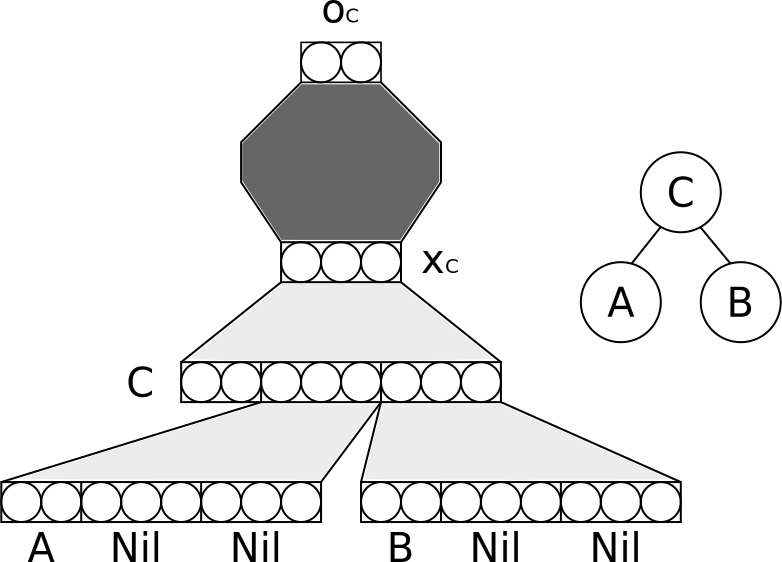
\includegraphics[scale=0.4]{img/virtual_unfolding}
	\caption{Virtual unfolding, reflecting the sample graph structure}
	\label{fig:virtual_unfolding}
\end{center}
\end{figure}

To explain the idea of BPTS it is necessary to briefly summarize the idea of BPTT (a detailed explanation can be found in RNN-concerned publications, e.g.~\cite{williams1995gradient}). Let's consider a fully-connected recurrent neural network, designed for classifying sequences of samples of size $m$. The network consists of a single layer of $n$ units with $n \times n$ recurrent connections, producing an output $\bm{y}(t)$ at time $t$. Let $\bm{x}^{s}(t)$ denote the $m$-tuple of input signals corresponding to the sample fed at time $t$. Further, let $\bm{x}(t)$ be the merged input fed to the network at time $t$, obtained by concatenating the vectors $\bm{x}^{s}(t)$ and $\bm{y}(t)$. To distinguish between the elements of vector $\bm{x}(t)$ corresponding to $\bm{x}^{s}(t)$ and to $\bm{y}(t)$, let's introduce two subsets of indices: $I$ and $U$ (Eq.~\ref{eq:bptt_indices}).

\begin{equation}
x_j(t) = \left\{
\begin{array}{l l}
	x^{s}_{j}(t)	& \quad \text{if $j \in I$} \\
	y_j(t)	& \quad \text{if $j \in U$}\\
\end{array} \right.
\label{eq:bptt_indices}
\end{equation}

\noindent Let $w_{kj}$ denote the network weight on connection to the $k$th neuron from input $x_j$, $net_k(t)$ denote the weighted sum of neuron inputs fed to the activation function of the $k$th neuron, $f_k$~(Eq.~\ref{eq:bptt_netk}) and $J(t)$ denote the overall mean square error of the network at time $t$.
\begin{equation}
net_k = \sum_{j \in (I \cup U)} w_{kj} x_j
\label{eq:bptt_netk}
\end{equation}

\begin{equation}
y_k = f_k(net_k)
\label{eq:bptt_f}
\end{equation}

\begin{equation}
J(t) = -\frac{1}{2} \sum_{k \in U} [e_k(t)]^2
\label{eq:bptt_j}
\end{equation}

\begin{equation}
e_k(t) = d_k(t) - y_k(t)
\label{eq:bptt_e}
\end{equation}

\noindent Let's consider a recurrent network which was operating from a starting time $t_0$ up to time $t$. We may represent the computation process performed by the network by \emph{unrolling} the network in time, that is building a feed-forward neural network made of identical instances of the considered recurrent neural network, one instance per time step $\tau$, $\tau \in (t_0, t]$. To compute the gradient of $J(t)$ at time $t$ it is necessary to compute values $\epsilon_k(\tau)$ and $\delta_k(\tau)$ for $k \in U$ and $\tau \in (t_0, t]$ by means of equations~\ref{eq:bptt_epsilon},~\ref{eq:bptt_delta} and~\ref{eq:bptt_summaric}.

\begin{equation}
\epsilon_k(t) = e_k(t)
\label{eq:bptt_epsilon}
\end{equation}

\begin{equation}
\delta_k(\tau) = f'_k(net_k(\tau))\epsilon_k(\tau)
\label{eq:bptt_delta}
\end{equation}

\begin{equation}
\epsilon_k(\tau - 1) = \sum_{j \in U} w_{jk} \delta_j(\tau)
\label{eq:bptt_summaric}
\end{equation}

\noindent Then, the gradient of $J(t)$ is calculated with respect to each weight $w_{ij}$ by the means of equation~\ref{eq:bptt_dj}.

\begin{equation}
\frac{\partial J(t)}{\partial w_{ij}} = \sum_{\tau = t_0 + 1}^{t} \delta_i(\tau) x_j(\tau - 1)
\label{eq:bptt_dj}
\end{equation}

\noindent At time $t$ an external error $\bm{e}(t)$ is \emph{injected} to the network, usually being the difference between the trained network output at time $t$: $\bm{y}(t)$ and the expected output $\bm{d}(t)$~(Eq.~\ref{eq:bptt_e}). The subsequent steps compute the error $\bm{\epsilon}(\tau)$ by backpropagating the original error through the layers of the unrolled neural network.

The BPTS method implements the BPTT algorithm. Backpropagation starts at the last layer of the virtual unfolding network, where the classification/regression error is calculated (the last layer of the transformation network applied to the root node). The error is injected to this layer and backpropagated using the BPTT algorithm down to the first layer of the folding network applied to the root node. The error is then backpropagated to the last layers of the folding network applied to the roots children, as if there was a physical connection. Such backpropagation continues down to the first layers of folding network applied to the terminal nodes.

The folding architecture model introduced new important ideas in the domain of connectionist graph processing models. First of all, the representation building model is simpler than the LRAAM model and the folding architecture converges much faster than LRAAM for the same datasets~\cite{goller1996learning}. Secondly, three important concepts were adapted from the domain of recurrent neural networks: the error injection, BPTS and the unfolding of the network as a generalisation of unrolling a recursive neural network.

\section{Generalised recursive neuron}
The \emph{generalised recursive neuron}, introduced in 1997~\cite{sperduti1997supervised} is a generalisation of the recurrent neuron, which in turn is used in recurrent neural networks (RNNs). It was created to provide an elementary component for the graph processing models which would be by definition better suited to solve graph processing tasks than the standard neuron. It is beyond the scope of this thesis to describe in detail the idea itself and its applications. Nevertheless this summary of the connectionist models would be incomplete without mentioning the generalised recursive neuron, as it was used in some of the following models instead of the common neural network neuron, yielding promising results~\cite{frasconi1998general}.

\noindent A generalised recursive neuron has two kinds of inputs:
\begin{itemize}
\item plain neuron inputs, which are fed with elements of the currently processed node label
\item recursive inputs, which are fed with the memorized output of the neuron for all children nodes of the currently processed node
\end{itemize}

\noindent In such a way, the neuron output changes after each training algorithm iteration, according to its output for all the children nodes.

\section{Recursive neural networks}
The folding architecture model had a large impact on a theory introduced in 1998, the \emph{structural transduction} formalism~\cite{frasconi1998general}. It is beyond the scope of this thesis to describe the formalism itself, let's mention however its aspects that highly affected the subsequent connectionist models described. The \emph{structural transduction}, in general, is a relation which maps a labelled DPAG (only node labels, no edge labels) into another DPAG. The type of transductions that the authors focus on are \emph{IO-isomorph} transductions, that is transductions that don't change the graph topology, only the node labels. (According to the authors managing transductions which are not \emph{IO-isomorph} is highly nontrivial and is an open research problem.) Let's describe an \emph{IO-isomorph} transduction. Let $G_s$ be the original DPAG with labelled nodes. Let $G_y$ be a graph with same topology that $G_s$ but with node labels replaced by expected node outputs for each node (it's a node classification/regression problem). A transduction $G_s \Rightarrow G_y$ can be described in terms of two functions, $f$ and $g$, where $f$ is the \emph{state transition function}, which builds the representation (the \emph{state}) $\bm{x}$ of the graph $G_s$ for the model and $g$ is the \emph{output function}, which produces the expected output graph $G_y$ according to the representation $\bm{x}$ and the original graph $G_s$. More precisely, for each node $i$ belonging to the original graph $G_s$ its state $\bm{x}_i \in \bm{x}$ and output ${\bm{y}}_i \in G_y$ are defined by Eq.~\ref{eq:recursive_state} and~\ref{eq:recursive_output}, where $\bm{l}_i$ is the $i$th node label and $\bm{x}_{ch[i]}$ is a vector obtained by stacking representations of all children of $i$th node one after another. In the original equations the $i$th node itself was also an argument of both functions, however, it was unnecessary from the point of view of recursive neural networks and therefore was omitted. 

\begin{equation}
\bm{x}_i = f(\bm{l}_i, \bm{x}_{ch[i]})
\label{eq:recursive_state}
\end{equation}

\begin{equation}
	\bm{y}_i = g(\bm{l}_i, \bm{x}_i)
\label{eq:recursive_output}
\end{equation}

The transduction can be implemented e.g. by a hidden recursive model (HRM) or by a \emph{recursive neural network} (a generalisation of a recurrent neural network, which is able to process not only sequences, but also DPAGs). In the case of a recursive neural network the functions $f$ and $g$ are implemented by two feed-forward neural networks. Identical instances of the $f$ network are connected according to the $G_s$ graph structure, creating the \emph{encoding network}. (The encoding network is the recursive neural network \emph{unfolded through the structure} of the given DPAG.) Calculation of the state $\bm{x}$ is performed by applying the $f$ network to the terminal nodes of $G_s$ and then proceeding up to the root, according to the encoding network topology. When the state calculation is finished, the $g$ network is applied to every node state $\bm{x}_i$, producing the requested output $\bm{y}_i$. A sample graph and the corresponding encoding network are presented in~Fig.~\ref{fig:recursive}.

\begin{figure}
\begin{center}
	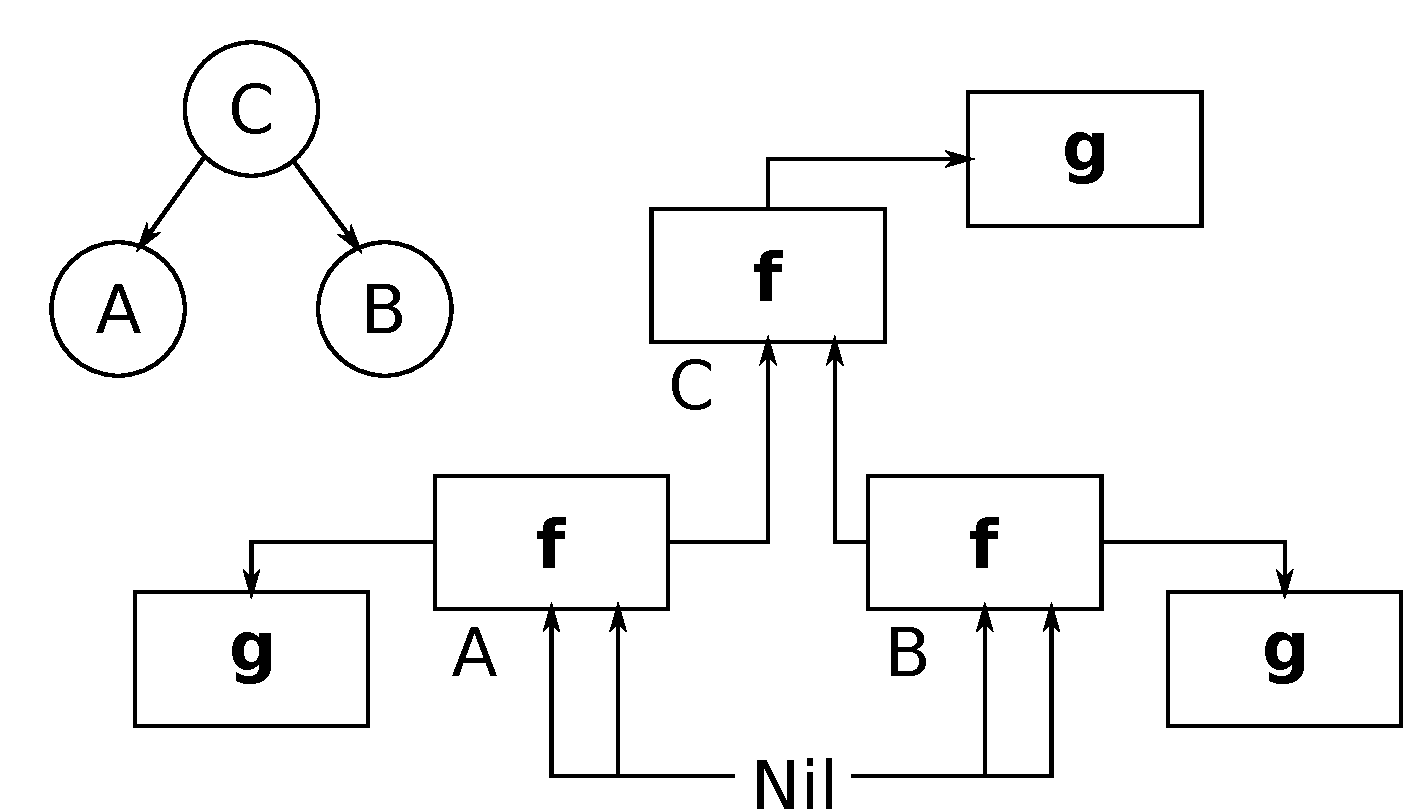
\includegraphics[scale=0.4]{img/encodinginc_recursive}
	\caption{A sample acyclic graph and the corresponding encoding network}
	\label{fig:recursive}
\end{center}
\end{figure}

As various kinds of neural network can be used as the $f$ function (first, second-order recurrent networks etc.), the recursive neural network model can become really complex and computationally powerful. However, for the scope of this work, it is sufficient to mention that the concepts of \emph{state transition function}, \emph{output function} and \emph{encoding network unfolded through structure} (originating from the \emph{folding architecture}) were later reused in the Graph Neural Network model. Another important feature of this model is a successful adaptation of ideas originating from recurrent neural network domain, just like in case of the \emph{folding architecture}. Authors of both models suggested that adaptation of other RNN ideas may also be possible, which could lead to novel graph processing solutions~\cite{kuchler1996inductive}~\cite{frasconi1998general}.
